\section{Сухое электронно-лучевое травление резиста}

Как было отмечено, в существующих методах микро- и нано-структурирования, основанных на термической деполимеризации резиста, нагрев резиста носит локальный характер -- как по времени, так и в пространстве. В отличие от них, в методе СЭЛТР резист остается полностью нагретым на протяжении всего процесса экспонирования. Глобальный характер нагрева резиста приводит к тому, что важным фактором, определяющим конечный профиль линии, становятся процессы термического растекания резиста. Здесь наблюдается определенное сходство с вышеописанным методом полутоновой литографии, дополненным стадией оплавления резиста для сглаживания рельефа. Однако, в методе СЭЛТР термическое растекание резиста протекает одновременно со всеми остальными процессами, включающими электронно-стимулированную термическую деполимеризацию резиста и диффузию мономера в слое резиста. Одновременное протекание всех процессов, определяющий конечный профиль линии, получаемой методом СЭЛТР, делает этот метод сложным для теоретического исследования. До настоящего времени метод СЭЛТР исследовался в большей степени экспериментально, и далее будут подробно описаны шаги, предшествовавшие настоящей работе.


\subsection{Цепная термическая деполимеризация полимеров}
В первых работах по изучению термической деполимеризации виниловые полимеры подвергались действию ультрафиолетового излучения при температурах выше их температуры стеклования (120--200~$^\circ$C)~\cite{Cowley_1952_1, Cowley_1952_2, Grassie1949_1, Grassie1949_2, Grassie1949_3, Grassie1949_4}.
Анализ распределения молекулярной массы облученных полимеров, получаемого методом гель-проникающей хроматографии, и продуктов распада позволил сделать вывод о цепном характере реакции деполимеризации полимера и получить оценки для средней длины кинетической цепи при деполимеризации.
Были определены процессы, протекающие при термической деполимеризации полимеров -- образование активного центра деполимеризации (инициирование кинетической цепи), его распространение вдоль молекулы (рост кинетической цепи) и возможный перенос на другую молекулу, а также затухание активного центра деполимеризации за счет различных эффектов (обрыв кинетической цепи).
Были предложены кинетические уравнения, учитывающие данные процессы, что позволило оценить значения констант процессов исходя из экспериментальных данных.

На рисунке~\ref{fig:Cowley_Mn} приведены зависимости отношения среднечисловой молекулярной массы облученного полимера ($\Mn$) к исходной среднечисловой молекулярной массе ($M_\mathrm{n0}$) от степени деградации полимера, полученные в работе~\cite{Cowley_1952_1}.
Было установлено, что для образцов высоким значением $M_\mathrm{n0}$ отношение $\Mn / M_\mathrm{n0}$ уменьшается практически линейно, в то время как для образцов с более низким значением $M_\mathrm{n0}$ данное отношение на начальных этапах деградации практически не изменяется.
Для обоснования этого явления было выдвинуто предположение о том, что реакция деполимеризации носит цепной характер.
Средняя длина кинетической цепи при деполимеризации при этом такова, что длинные молекулы распадаются не до конца, что приводит к изменению $\Mn$.
В то же время короткие (относительно средней длины кинетической цепи при деполимеризации) молекулы распадаются полностью, что исключает их вклад в значение $\Mn$.

\begin{figure}[t]
	\centering
	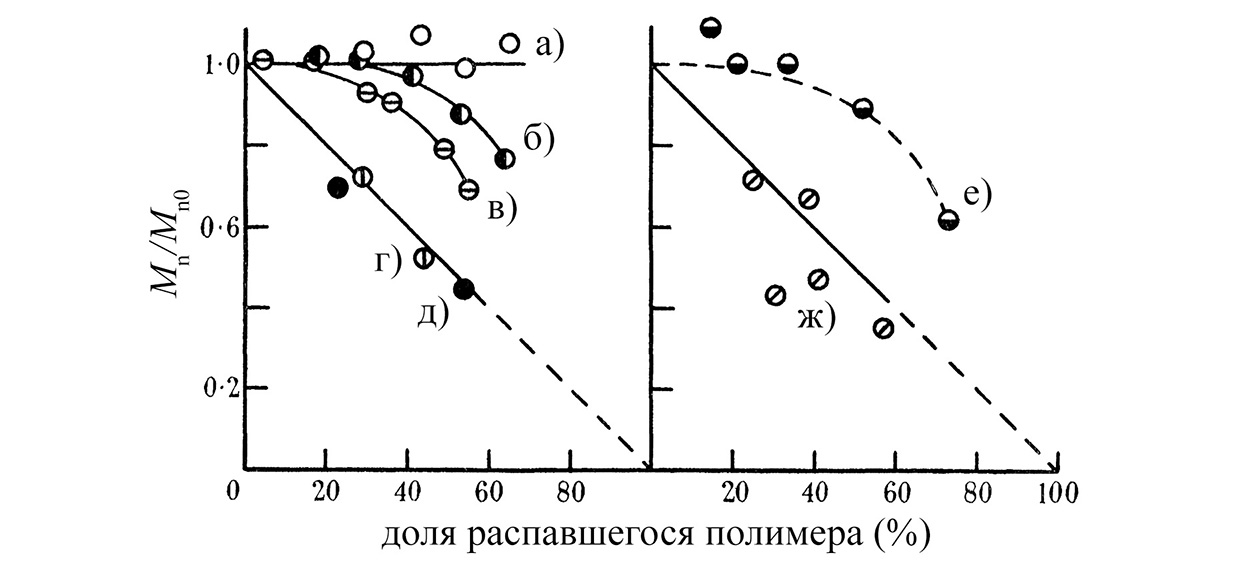
\includegraphics{1_chapter/Cowley_Mn_14pt_200}
	\vspace{0.5em}
	\caption{Зависимости отношения $\Mn / M_\mathrm{n0}$ от доли распавшегося полимера при термической деполимеризации полиметилметакрилата для различных значений $M_\mathrm{n0}$: a) 44300, б) 94000, в) 179000, г) 650000, д) 725000, е)~125000, ж) 770000~\cite{Cowley_1952_1}.}
	\label{fig:Cowley_Mn}
\end{figure}

Последующие исследования на основе Фурье-спектроскопии позволили более детально описать процесс термической деполимеризации.
Так, например, анализ интенсивности отдельных полос спектра, соответствующих различным связям в полимерной молекуле, позволил определить основные механизмы радиационно-стимулированной деполимеризации~\cite{Bermudez} (см. рисунок~\ref{fig:PMMA_degpaths}).
В дальнейшем наиболее полная картина процессов термической деполимеризации была сформирована уже за счет применения методов молекулярной динамики~\cite{Stoliarov}.

\begin{figure}[t]
	\centering
	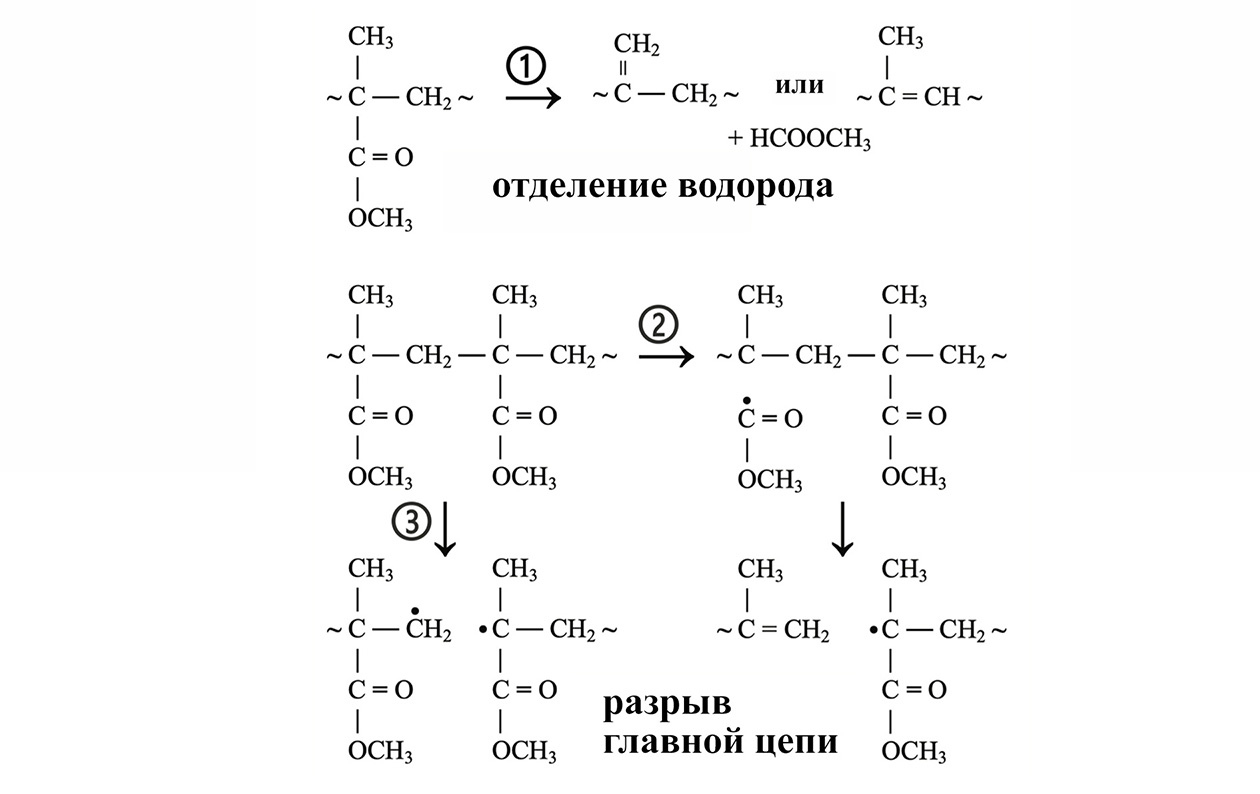
\includegraphics{1_chapter/PMMA_degpaths_14pt_200}
	\caption{Схематическое изображение основных механизмов разрыва молекул ПММА при воздействии внешнего излучения~\cite{Bermudez}.}
	\label{fig:PMMA_degpaths}
\end{figure}

Важной особенностью термической деполимеризации является тот факт, что энергия активации процесса термического образования активного центра деполимеризации выше энергии активации процесса его распространения вдоль полимерной молекулы~\cite{Cowley_1952_1, Sanchez-Jimenez_Ea}.
Это означает, что существует область температур, в которой реакция цепной термической деполимеризации может протекать только при условии, что активный центр деполимеризации был образован по механизму, отличному от термического.
Таким механизмом может являться, например, локальное воздействие внешнего излучения.
Это приводит к концепции метода микролитографии на основе реакции цепной термической деполимеризации, инициируемой внешним излучением в слое резиста, нагретом до температуры, превышающей температуру стеклования резиста.
Первое упоминание о возможности такого метода микролитографии встречается в работе, посвященной ионно-стимулированной термической деполимеризации полиметилметакрилата \linebreak (ПММА)~\cite{Fragala_1}.
В последующих работах этого автора была изложена подробная модель образования и выхода мономера из слоя \linebreak ПММА при ионно-стимулированной термической деполимеризации~\cite{Fragala_2,Fragala_3_diffusion}, \linebreak однако, к идее метода микролитографии на основе термической деполимеризации он уже не возвращался.


%\subsection{Развитие метода микролитографии на основе термической деполимеризации резиста}
\subsection{Развитие метода сухого электронно-лучевого травления резиста}
Первые шаги в изучении метода микролитографии на основе радиационно-стимулированной термической деполимеризации резиста описываются в работе~\cite{Bruk_2000}. В ней приводятся результаты инициированной $\gamma$-излучением деполимеризации ПММА в виде нанометрового слоя, адсорбированного на поверхности пор силохрома. Несмотря на то, что в данной работе термическая деполимеризация не использовалась для формирования структуры в резисте, а исследовалась в общем, результаты работы позволили определить особенности потенциально возможного метода микроструктурирования на основе этого явления. Так, например, были получены оценки для времени диффузии мономера в слое ПММА после разрушения молекулы и средней длины кинетической цепи при деполимеризации, а также были сделаны выводы о масштабах протекания процессов передачи активного центра деполимеризации на мономер и полимер. Помимо этого было установлено, что при радиационно-стимулированной термической деполимеризации ПММА в области температур 120--180~$^\circ$C влияние процессов реполимеризации пренебрежимо мало.

Впоследствии были проведены эксперименты по изучению термической деполимеризации ПММА, протекающей при его экспонировании электронным лучом, а также впервые были продемонстрированы двумерные и трехмерные структуры, полученные в этом процессе~\cite{Bruk_2013}. Такой метод формирования рельефа в резисте получил название СЭЛТР -- сухое электронно-лучевое травление резиста. Методика экспериментов была следующей:
\begin{enumerate}
	\item На пластину монокристаллического кремния методом ``spin-coating'' из 2\%-ного раствора в анизоле с последующей сушкой наносили слой \linebreak ПММА (PMMA 950K A2 от компании ``Allresist'') толщиной \linebreak $L_0$ = 80-85~нм;
	\item Полученные образцы помещали на специальный нагреватель, вводили в камеру электронного микроскопа Camscan S-4 или Zeiss Ultra-55, разогревали до нужной температуры и в вакууме порядка 10$^\text{-5}$ мбар подвергали экспонированию электронным лучом в режиме сканирования ``в~кадр'' либо вдоль линии;
	\item После экспонирования нагревательный элемент отключался, и резист остывал в камере электронного микроскопа в вакууме естественным образом;
	\item Толщина слоя ПММА до и после процесса СЭЛТР, а также профиль получаемого рельефа определялись методом атомно-силовой микроскопии с использованием микроскопа Solver P47-SPM-MTD.
\end{enumerate}

Начальная энергия электронного пучка, ток экспонирования и диаметр электронного пучка составляли примерно 20 кэВ, 1 нА и 600 нм соответственно для электронного микроскопа Camscan S-4 и 15 кэВ, 1.5 пА и 10 нм соответственно для электронного микроскопа Zeiss Ultra-55.

Одним из важных результатов работы стали кинетические кривые травления в методе СЭЛТР -- зависимости нормализованной толщины слоя резиста $L_\mathrm{norm} = L/L_0$ от дозы экспонирования (рисунок~\ref{fig:kin_curves}). Было установлено, что дозы полутравления $D_\text{0.5}$ (дозы, при которой толщина слоя ПММА уменьшается вдвое относительно начальной толщины) составляют приблизительно 2.5, 0.8 и 0.3 мкКл/см$\pp$ для температур 125, 150 и 170~$^\circ$C соответственно. Дозы полного травления слоя резиста $D_\text{1}$ для этих же температур составили приблизительно 20, 12 и 6.5 мкКл/см$\pp$. Таким образом, дозы $D_\text{1}$ примерно в 10 раз (а дозы полутравления -- в 100 раз) меньше доз, необходимых для формирования рельефа в ПММА методом обычной электронно-лучевой литографии (для которой $D_\text{1}$ составляет порядка 100 мкКл/см$\pp$).

\begin{figure}[h]
	\centering
	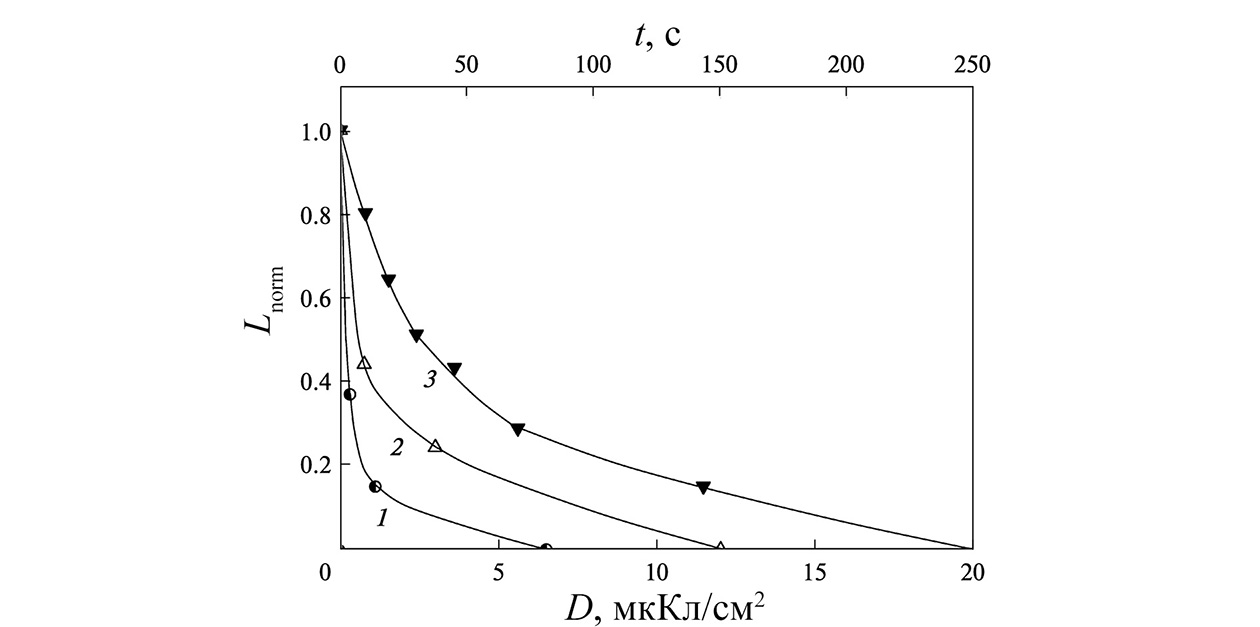
\includegraphics{1_chapter/DEBER_kin_curves_14pt_200}
	\vspace{0.5em}
	\caption{Кинетические кривые травления ПММА в методе СЭЛТР, полученные для температур 125 (1), 150 (2) и 170~$^\circ$С (3)~\cite{Bruk_2013}.}
	\label{fig:kin_curves}
\end{figure}

Было выдвинуто предположение, что в проведенных опытах формирование рельефа обеспечивалось за счет объемной релаксации полимера, протекавшей достаточно быстро по сравнению с характерным временем всего эксперимента.
Более того, считалось, что скорость травления была пропорциональна толщине слоя ПММА и уменьшалась в ходе процесса за счет уменьшения последней.
Также предполагалось, что в проведенных опытах диффузия образующегося в слое резиста мономера протекала достаточно быстро для того, чтобы процессы диффузии не ограничивали скорость травления.
Для обоснования этого предположения было введено понятие приведенной скорости травления $W_\mathrm{red}$, равной отношению средней скорости травления в некоторой точке кинетической кривой ($V_\mathrm{i}$) к толщине слоя ПММА, соответствующей этой точке ($L_\mathrm{i}$):
\begin{equation}
	W_\mathrm{red} = V_\mathrm{i} / L_\mathrm{i}.
\end{equation}

На рисунке~\ref{fig:DEBER_W} приведена зависимость $W_\mathrm{red}$ от нормализованной толщины слоя ПММА в ходе процесса СЭЛТР при 125~$^\circ$С. Характер этой зависимости показывает, что даже в начале процесса, когда толщина слоя максимальна, диффузия мономера из слоя резиста протекает достаточно быстро и не влияет на скорость травления. В самом деле, если бы диффузия мономера замедляла процесс травления, то $W_\mathrm{red}$ должна была бы возрастать, поскольку время диффузионного проскока молекул газа $\tau_\mathrm{diff}$ пропорционально квадрату толщины слоя $l$, через который происходит диффузия~\cite{Bruk_2000}:
\begin{equation}
	\tau_\mathrm{diff} = l^2 / 12 D,
\end{equation}
где $D$ -- эффективный коэффициент диффузии газа.

Из рисунка~\ref{fig:DEBER_W} видно, что величина $W_\mathrm{red}$ остается постоянной вплоть до значений конверсии около 50\%, после чего начинает уменьшаться. Наблюдаемое уменьшение $W_\mathrm{red}$ могло быть связано с уменьшением молекулярной массы ПММА и (или) с возникновением в нем в ходе экспонирования дополнительных дефектов, ускоряющих обрыв кинетической цепи при деполимеризации.

\begin{figure}[b]
	\centering
	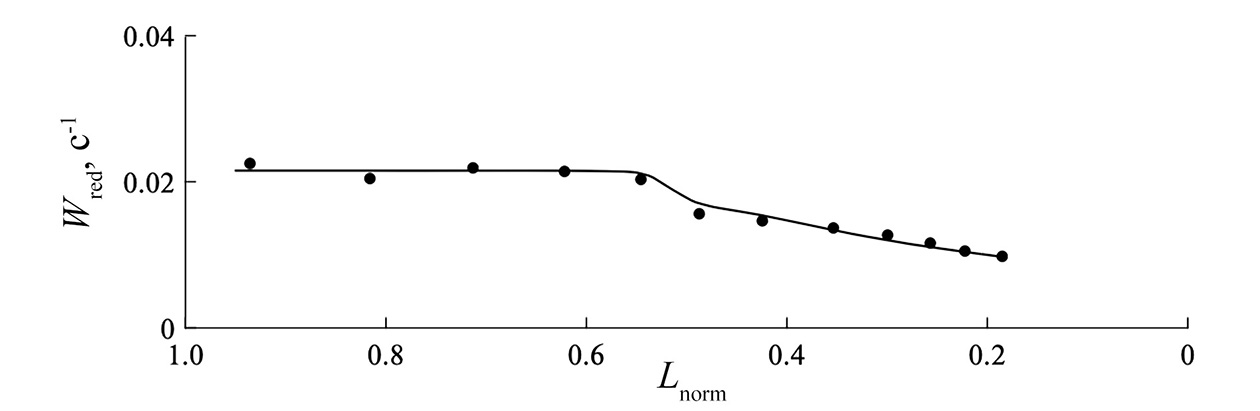
\includegraphics{1_chapter/DEBER_W_14pt_200}
	\vspace{0.2em}
	\caption{Зависимость приведенной скорости травления $W_\mathrm{red}$ для ПММА в методе СЭЛТР при температуре 125~$^\circ$C~\cite{Bruk_2013}.}
	\label{fig:DEBER_W}
\end{figure}

Также в работе~\cite{Bruk_2013} были проведены первые опыты по формированию методом СЭЛТР трехмерных ступенчатых структур -- на кремниевой пластине со слоем резиста, разогретыми до необходимой температуры, при неизменном положении пластины производили последовательно несколько экспонирований по последовательно сужающимся квадратным площадкам (рисунок~\ref{fig:DEBER_stairs}). Соотношение линейных размеров площадей сканирования определяло ширину ступеней формирующихся на краю экспонируемой области. Дозы облучения при каждом экспонировании рассчитывались в соответствии с кинетической кривой травления, при этом для каждого последующего экспонирования учитывалась доза, полученная экспонируемой областью ранее. При этом была отмечена достаточно высокая однородность травления по оси $Z$: шероховатость ступенек шириной 5–10 мкм по оси $Z$ составляла всего около 1–2 нм.
Было также отмечено низкое аспектное отношение получаемых структур -- угол наклона стенок профиля относительно горизонтали составлял около 3$^\circ$. Было предположено, что основными причинами этого явления являются специфическая форма кинетической кривой травления в методе СЭЛТР и пониженная вязкость ПММА в условиях процесса СЭЛТР, приводящая к растеканию рельефа.

\begin{figure}[h]
	\centering
	\vspace{0.2em}
	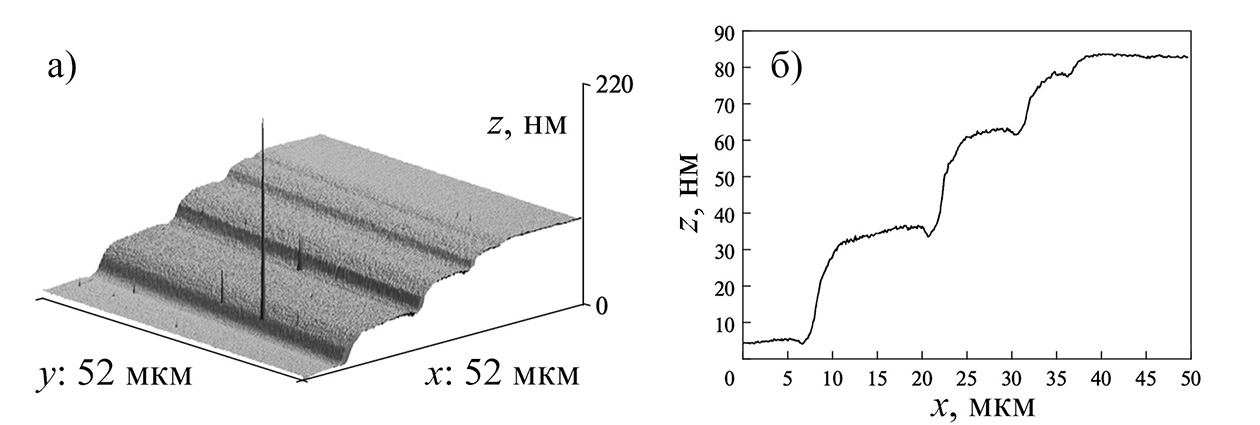
\includegraphics{1_chapter/DEBER_stairs_14pt_200}
	\vspace{0.5em}
	\caption{Ступенчатые профили, полученные в слое ПММА методом СЭЛТР путем экспонирования по последовательно сужающимся квадратным площадкам при температуре 125~$^\circ$C~\cite{Bruk_2013}. \vspace{1.5em}}
	\label{fig:DEBER_stairs}
\end{figure}


\subsection{Текущая стадия разработки метода сухого электронно-лучевого травления резиста}

Наиболее актуальные на сегодняшний день результаты экспериментальных исследований метода сухого электронно-лучевого травления резиста приведены в работах~\cite{Bruk_2015_co, Bruk_2016_mee}. Помимо вышеописанных ступенчатых профилей, в этих работах исследовались периодические профили, полученные при экспонировании резиста электронным лучом вдоль серии параллельных линий (рисунок~\ref{fig:DEBER_many_profiles}). Было продемонстрировано, что при таком экспонировании результирующий профиль имеет форму, близкую к синусоидальной, что является аргументом в пользу использования метода СЭЛТР для формирования различных дифракционных и голографических оптических элементов~\cite{Mitreska_sin_gratings}. При этом снова была отмечена высокая производительность метода -- при температуре 160~$^\circ$C полное травление в центре линии достигалось при дозе экспонирования менее 1 мкКл/см$\pp$. Также была продемонстрирована возможность переноса профиля, полученного методом СЭЛТР в ПММА, в вольфрам и кремний путем травления в реакторе индуктивно-связанной плазмы (рисунок~\ref{fig:DEBER_Si_W}). За счет этого одной из возможных областей применения метода СЭЛТР может быть формирование штампов для термической НИЛ.

\begin{figure}[h]
	\centering
	\vspace{0.2em}
	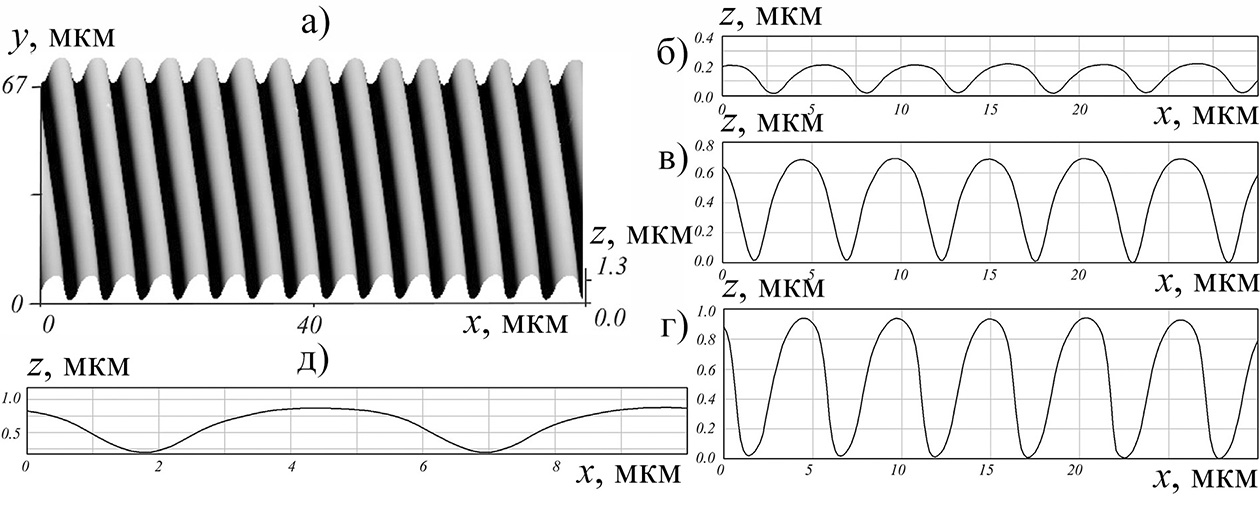
\includegraphics{1_chapter/DEBER_many_profiles_14pt_200}
	\vspace{0.2em}
	\caption{Профили периодических структур, полученных методом СЭЛТР в слое ПММА толщиной 900 нм при экспонировании вдоль серии параллельных линий при температуре 160~$^\circ$C: а) трехмерное изображение; б), в), г) профили, полученные при дозах экспонирования 0.05, 0.2 и 0.87 мкКл/см$\pp$ соответственно, д) изображение профиля в) в масштабе 1:1~\cite{Bruk_2016_mee}.}
	\label{fig:DEBER_many_profiles}
\end{figure}

\begin{figure}[t]
	\centering
	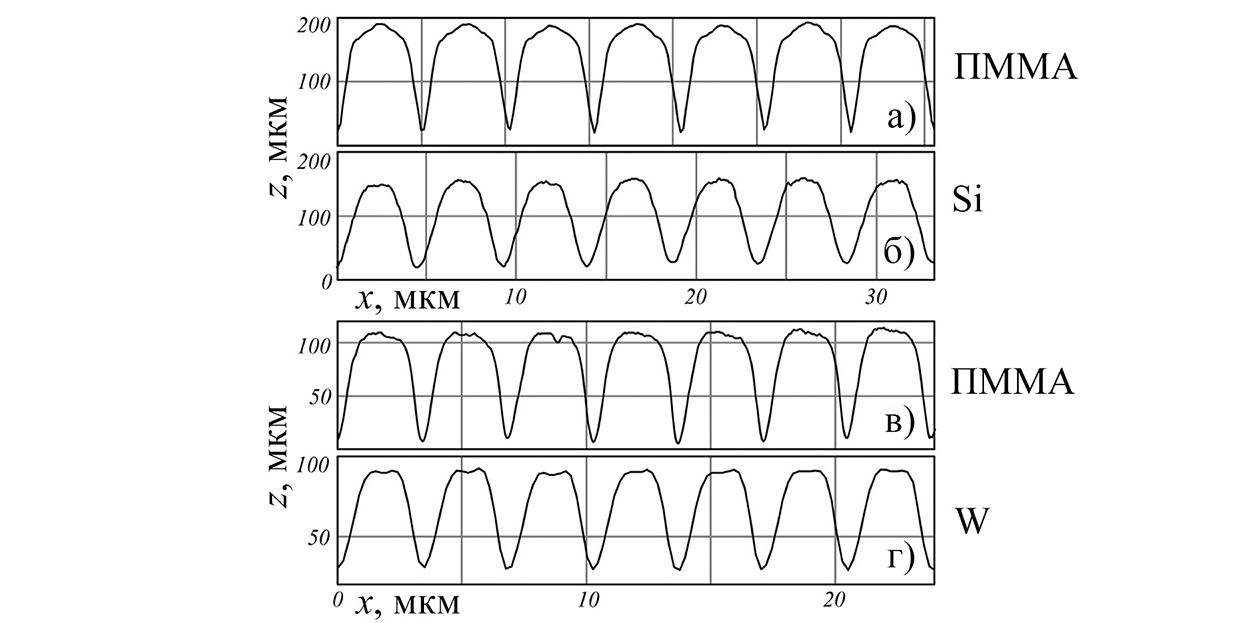
\includegraphics{1_chapter/DEBER_Si_W_14pt_200}
	\vspace{0.2em}
	\caption{Сечения профилей структур, полученных методом СЭЛТР в слое ПММА до (а) и в)) и после (б) и г)) переноса в кремний (Si) и вольфрам (W)~\cite{Bruk_2016_mee}.}
	\label{fig:DEBER_Si_W}
\end{figure}

Для оценки величины латерального разрешения метода СЭЛТР были исследованы профили, полученные при экспонировании резиста остросфокусированным электронным пучком вдоль одиночных линий (рисунок~\ref{fig:DEBER_Ultra}).
При использовании пучка с диаметром около 10 нм ширина одиночных линий на полувысоте составила примерно 300 нм, что было принято за предельное разрешение метода СЭЛТР.

Резюмируя все вышесказанное, можно выделить преимущества и недостатки метода СЭЛТР.
К преимуществам данного метода относятся:
\begin{itemize}
	\item высокая производительность, обеспечиваемая реакцией цепной термической деполимеризации резиста -- характерные дозы, необходимые для формирования рельефа методом СЭЛТР в десятки раз меньше, чем характерные дозы при обычной электронно-лучевой литографии;
	\item относительная простота метода -- для формирования дву- и трехмерных структур в резисте требуется всего одна вакуумная стадия;
	\item возможность реализации в различных электронно-лучевых системах -- метод СЭЛТР может быть реализован в растровых электронных микроскопах, электронных литографах и других электронно-лучевых системах с минимальными модификациями (обеспечение возможности нагрева образца и, при необходимости, установка ловушек для мономера);
	\item сглаженный профиль получаемых структур, обеспечиваемый процессами растекания.
\end{itemize}

\begin{figure}[t]
	\centering
	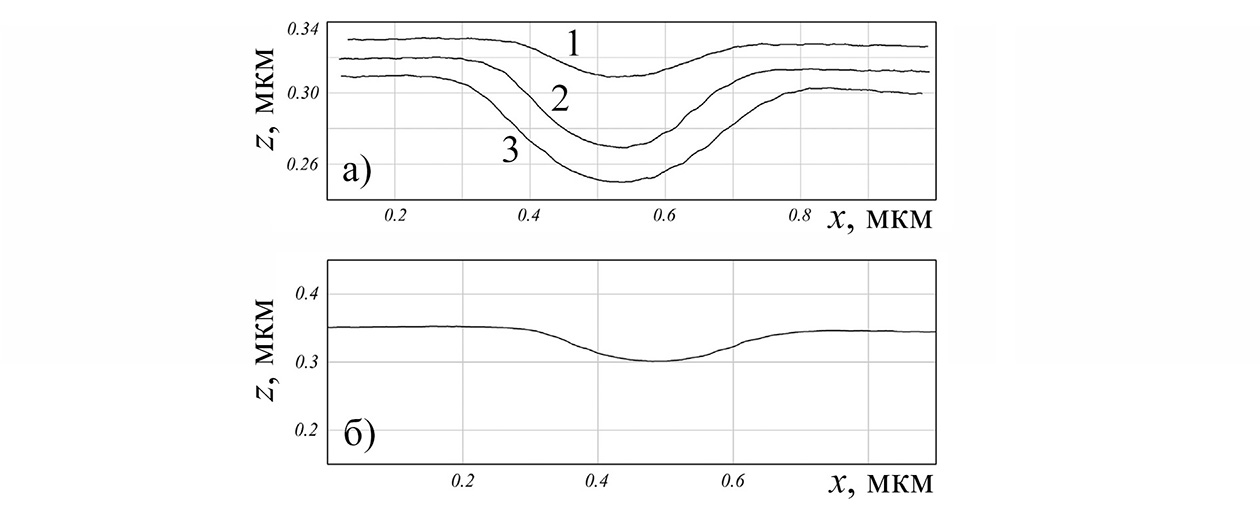
\includegraphics{1_chapter/DEBER_Ultra_14pt_200}
	\caption{а) Профили одиночных линий, полученных методом СЭЛТР в слое ПММА толщиной 80 нм при экспонировании остросфокусированным электронным пучком (диаметр пучка составляет около 10 нм) при температуре 116~$^\circ$C. Время экспонирования составляло 1, 4 и 16 с (профили 1, 2 и 3 соответственно); б) Изображение профиля 2 в масштабе 1:1~\cite{Bruk_2016_mee}.}
	\label{fig:DEBER_Ultra}
\end{figure}

При этом, в настоящее время главными недостатками метода СЭЛТР являются низкое латеральное разрешение и низкое аспектное отношение получаемых структур.
До настоящего времени при использовании электронно-лучевых систем с диаметром луча около 10~нм методом СЭЛТР удавалось получать канавки c минимальной шириной на полувысоте около 300 нм и максимальным углом наклона стенок около 20$^\circ$.
В силу одновременного протекания при СЭЛТР множества различных процессов точный механизм формирования конечного профиля линии не был понятен, что не позволяло выявить пути оптимизации данного метода.
Экспериментальные исследования процесса СЭЛТР, проводившиеся до настоящего времени, ограничивались лишь изучением конечного профиля получаемых структур.
Такой подход не позволял определить вклад отдельных процессов в латеральное разрешение метода СЭЛТР, что существенно затрудняло его оптимизацию.
В то же время, при наличии физической модели метода СЭЛТР определение путей оптимизации метода и границ его применимости стало бы вполне возможным.
Построение такой модели могло бы быть основано на выделении основных процессов, влияющих на профиль линии в методе СЭЛТР, разработке их физических моделей на основе существующих подходов и дальнейшем объединении моделей отдельных процессов в модель процесса СЭЛТР в целом.
